\documentclass[letterpaper,titlepage,10pt]{article}
\usepackage[utf8]{inputenc}
\usepackage{amsmath}
\usepackage{amssymb}
\usepackage{graphicx}
\usepackage{epstopdf}
\usepackage{caption}
\usepackage{subcaption}
\usepackage{afterpage}
\usepackage{float}
\usepackage[left=2.5cm,top=3cm,right=2.5cm,bottom=3cm,bindingoffset=0.5cm]{geometry}
\title{Non-Linear Ordinary Differential Equations and Lorenz's Simplified Model for Fluid Convection}
\author{Alexis Tavares}
\date{AMAT 311}
\begin{document}
\maketitle{}
\tableofcontents{}
\newpage

\section{Preamble}
Up until the 1950's, atmospheric phenomena including meteorological events were described using linear statistical models. However one meteorologist, Edward Norton Lorenz (May 23rd 1917 - Apr. 16. 2008) was skeptical of these models as phenomena, particular those appearing in weather forecasting, tended to behave non-linearly.  His exposition into the matter led him to develop a  simple system of non-linear differential equations as a model for air movement in Earth's atmosphere and in studying these movements he noticed that they did not always move as predicted. Minimal changes in the initial values of his system resulted in divergent behavior patterns, and indicated that weather predictions that advanced much further than roughly a week were likely to be inaccurate.  He observed that his very simple system had very complex behavior and by extension the real world phenomena modeled by the system also could exhibit such behavior. \newline \newline
Lorenz, who was interested in creating accurate, long-term weather predictions, came to the conclusion that even something as seemingly insignificant as the flap of a butterfly's wings can have an influence on weather on the other side of the globe. This implied that others who attempted to model the Earth's climate would have to account for even the most minute fluctuations in weather in order to be accurate. With the advent of modern computers, the weather forecasting models of today can have up to a million unknown variables, yet Lorenz found, with even a simple system with considerably fewer variables, that long term behavior was just as unpredictable. He noted that this non-periodic or chaotic behavior appears in systems that can be described by non-linear differential equations. \newline \newline
Herein we attempt to understand how and why Lorenz came up with his system,its applications to weather and hydrodynamic systems as well as extensions of the system and their properties.

\section{The Lorenz System}
\subsection{Rayleigh-Bernard Convection}
{\parindent0pt
The Earth's atmosphere is one of many hydrodynamical systems that exhibits a variety of solution behavior. Some  sytems exhibit steady flow, some oscillate between at least two states and others vary in an irregular manner. The latter type of behavior in a fluid, in more general systems, is known as Chaos, the strong dependence of the solution on the initial conditions or the large divergence in solutions for small difference in the initial conditions.  An example of such behavior in physicals systems is thermal convection in fluids. \newline 

Lorenz's system is a simple model for a particular type of convention, Rayleigh-Bernard Convection, wherein fluid motion is induced by density differences in a horizontal fluid layer occurring due to the creation of temperature gradients.\cite{e} When the fluid is heated from below a pattern of convention cells (Bernard cells) occurs in a relatively shallow layer. On Earth this is roughly the first 2km of our atmosphere.\cite{d} The resulting temperature gradients can cause convection rolls where the hot fluid from below rises and the cold fluid above sinks in a cyclical manner. 
}
\subsection{Lorenz's Simplified model}
Lorenz's Model\cite{pa} for convection can be given as \cite{b}:

\begin{align*}
\dot{x} &= \sigma(y-x) \\
\dot{y} &= rx -y - zx  \\
\dot{z} &= -\beta z + xy 
\end{align*}

{\parindent0pt
Which is a non-linear ODE, where
\begin{flushleft}
\begin{verse}
$x$ represents velocity\\
$y$ and $z$ the temperature of the fluid \\
$r$, $\sigma$, $\beta$, positive parameters determined heating, physical fluid properties and height of the fluid layer.
\end{verse}
\end{flushleft}

In particular\cite{b}:
\begin{flushleft}
\begin{verse}
$r$ is the \textbf{Rayleigh number}, a measure of the temperature difference across the fluid layer \\
$\sigma$ the \textbf{Prandtl number}, the ratio of  coefficients of viscosity and thermal diffusion of the fluid and \\
$\beta$ is related to the frequency of oscillations in the field
\end{verse}
\end{flushleft}
}

\subsection{Solutions of the System}
{\parindent0pt
The Lorenz system is an initial value problem with a three dimensional ($y$ = \{$y_{1}$,$y_{2}$,$y_{3}$\}) ordinary differential equation system. It can be solved by the 4th order Runge-Kutta method.\cite{a}
Given our system:
\begin{align*}
\dot{x} &= \sigma(y-x) \\
\dot{y} &= rx -y - zx  \\
\dot{z} &= -\beta z + xy 
\end{align*}

We can re-write it as \cite{f}:
\begin{align*}
\frac{\text{dW}}{\text{d}x} &= Pr(T_{1}-W) \\
\frac{dT_{1}}{\text{d}x} &= -WT_{2} + rW - T_{1} \\
\frac{dT_{2}}{\text{d}x} &= WT_{1} - \beta T_{2}
\end{align*}

where $\beta$ = $\frac{4}{1+a^{2}} $ and $r$ = $\frac{Ra}{Ra_{c}}$ with $Ra_{c}$ the critical Raleigh number. \newline \newline
It is worth mentioning that there are very few known methods for solving non-linear differential equations. Non-linear differential equations have a tendency to produce very complicated behavior and can be characteristically chaotic. Even very fundamental properties like uniqueness, existence are very difficult questions. Solving these problems is considered to be an important advancement in mathematical theory. However, for non-linear equations that are analogous to meaningful real world concepts, we would expect to be able to find a solution. 
In Lorenz's case there is a solution to be found and it is found best by identifying W, $T_{1}$ and $T_{2}$ as $y_{1}$,$y_{2}$,$y_{3}$ and using Matlab for a 4th order Runge-Kutta scheme where the method works by using \cite{f}
\begin{align*}
y_{i+1} = y_{i} + \frac{1}{6}(k_{1}+2k_{2}+2k_{3}+k_{4})h
\end{align*}
with
\begin{align*}
k_{1} &= f(x_{i},y_{i}) \\
k_{2} &= f(x_{i}+ \frac{1}{2}h, y_{i}+ \frac{1}{2}k_{1}h) \\
k_{3} &= f(x_{i}+ \frac{1}{2}h, y_{i}+ \frac{1}{2}k_{2}h) \\
k_{4} &= f(x_{i}+ h, y_{i}+ k_{3}h)
\end{align*}
Where knowing the value of $y= y_{i}$ at $x_{i}$, we can find the value of $y=y_{i+1}$ at $x_{i+1}$ and $h=x_{i+1} - x_{i}$.  
And thus some solutions are given on the following page:
\newpage{}
\vfill 
\begin{figure}
        \centering
        \begin{subfigure}[H]{0.3\textwidth}
                
\includegraphics[width=\textwidth]{/home/deo/documents/amat311/p13.eps}
                \caption{r=13, $\sigma$=10, $\beta$ =$\frac{8}{3}$ }
                \label{fig:gull}
        \end{subfigure}%
      \quad
        ~ %add desired spacing between images, e. g. ~, \quad, \qquad etc.
          %(or a blank line to force the subfigure onto a new line)
        \begin{subfigure}[H]{0.3\textwidth}
                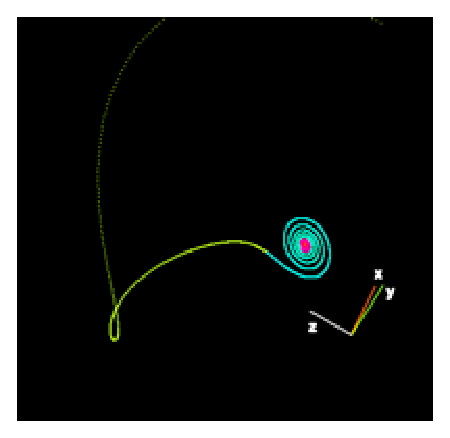
\includegraphics[width=\textwidth]{/home/deo/documents/amat311/p14-png.eps}
                \caption{r=14, $\sigma$=10, $\beta$ =$\frac{8}{3}$}
                \label{fig:tiger}
        \end{subfigure}
        \qquad \qquad
        ~ %add desired spacing between images, e. g. ~, \quad, \qquad etc.
          %(or a blank line to force the subfigure onto a new line)
        \begin{subfigure}[H]{0.3\textwidth}
                
\includegraphics[width=\textwidth]{/home/deo/documents/amat311/p15-png.eps}
                \caption{r=15, $\sigma$=10, $\beta$ =$\frac{8}{3}$}
                \label{fig:mouse}
        \end{subfigure}
        \quad
        \begin{subfigure}[H]{0.3\textwidth}
                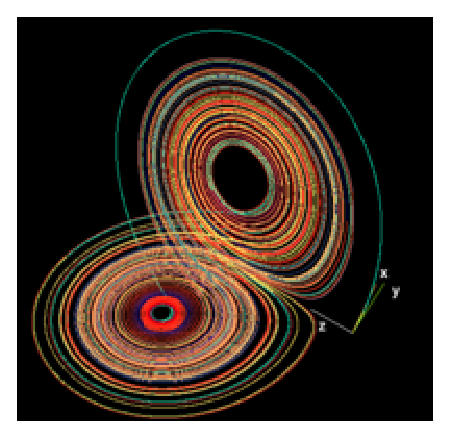
\includegraphics[width=\textwidth]{/home/deo/documents/amat311/p28-png.eps}
                \caption{r=28, $\sigma$=10, $\beta$ =$\frac{8}{3}$}
                \label{fig:mouse}
        \end{subfigure}
        \caption{Solutions for differing values of r \cite{c}}\label{fig:animals}
\end{figure}

\begin{figure}
        \centering
        \begin{subfigure}[H]{0.3\textwidth}
                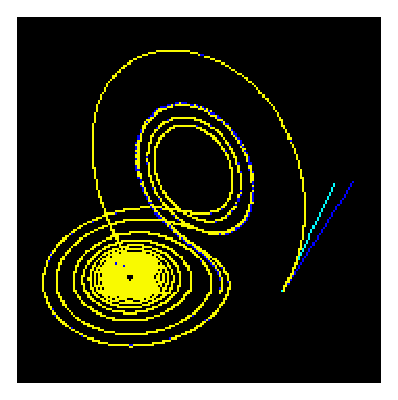
\includegraphics[width=\textwidth]{/home/deo/documents/amat311/tis1-png.eps}
                \caption{Time t=1}
                \label{fig:gull}
        \end{subfigure}%
        ~ %add desired spacing between images, e. g. ~, \quad, \qquad etc.
          %(or a blank line to force the subfigure onto a new line)
        \begin{subfigure}[H]{0.3\textwidth}
                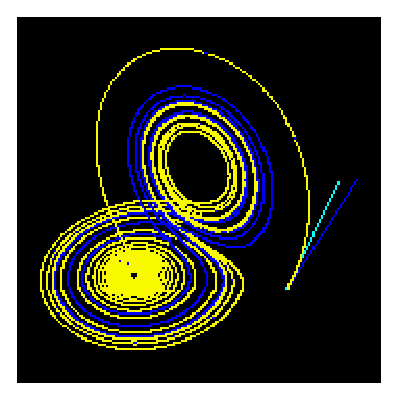
\includegraphics[width=\textwidth]{/home/deo/documents/amat311/tis2-png.eps}
                \caption{Time t=2}
                \label{fig:tiger}
        \end{subfigure}
        ~ %add desired spacing between images, e. g. ~, \quad, \qquad etc.
          %(or a blank line to force the subfigure onto a new line)
        \begin{subfigure}[H]{0.3\textwidth}
                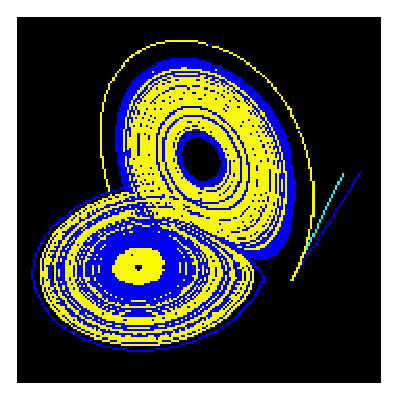
\includegraphics[width=\textwidth]{/home/deo/documents/amat311/tis3-png.eps}
                \caption{Time t=3}
                \label{fig:mouse}
        \end{subfigure}
        
        \caption{Solutions for differing values of t with r=28 \cite{c}}\label{fig:animals}
\end{figure}
\vfill
\clearpage
}

\subsection{Analysis of the System}
{\parindent0pt
Lorenz was particularly interested in the systems parameters r=28, $\sigma$ =10, $\beta$ = $\frac{8}{3}$ since, as shown in figure 2, the system exhibits chaotic behavior for these system parameters. The system has some interesting properties. The equations are invariant under the transformations S(x,y,z) = (-x,-y,z) \cite{b}, meaning that if (x(t), y(t), z(t)) is a solution then (-x(t),-y(t), z(t)) is also a solution.  If ($x_{0},y_{0},z_{0}) = (0,0,z_{0}$) then the equations become 
\begin{align*}
\dot{x} &= 0 \\
\dot{y} &= 0 \\
\dot{z} &= -\beta z
\end{align*}

Thus the system stays on the z-axis and to the equilibrium point (0,0,0). An equilibrium point being a point $x_{0}$ in $\mathbb{R}^{n}$ such that for $\frac{\text{dx}}{\text{d}t}$ = F(x) , $F(x_{0})$ = 0 \cite{g}. Thus, two other equilibrium points arise $C^{\pm} = (\pm\sqrt{\beta (r-1)}, \pm\sqrt{\beta (r-1)}, r-1) $ but for r $<$ 1 , all solutions are attracted to the origin. For $r>1$  there is a pair of fixed points $C^{\pm}$ at $x^{*}$=$y^{*}$ = $\pm\sqrt{\beta (r-1)}$, $z^{*}= r-1$. These coalesce with the origin as r approaches 1 from the positive direction in a pitchfork bifurcation. \cite{b} \newline \newline 
A bifurcation is a qualitative change in an attractor's structure as a system control parameter is varied. \cite{h} An attractor being the physical properties a system tends to evolve towards. \cite{h} With an equilibrium point serving as a fixed-point attractor (as in Lorenz's scenario), the attractor might create periodic oscillation  or  become unstable and be replaced by a chaotic attractor both of which Lorenz observed depending on the parameters used on his system. When his system was observed to become chaotic(As show in Figure 2d) \cite{b}, some characteristics could be observed:

\begin{description}
  \item[First] \hfill \\
  Long term behavior is difficult or impossible to predict. The system has to measured over and over again to find where it will be next because even very accurate measurments of the current state become terrible indicators of the future state. 
  \item[Second] \hfill \\
  There is a hypersensitive dependendance on initial conditions.. The system quickly moves to different states from relatively close initial conditions.
  \item[Third] \hfill \\
  Amplification errors occur when translating the system into a real world scenario (giving an experimenter the perception that the scenario is chaotic in nature).
\end{description}

These properties are what makes something "chaotic" fundamentally. By Poincare-Bendixson theorem \cite{j} since a 2 dimensional differential equation must have regular behavior, it cannot have a strange attrator and therefore cannot be chaotic. As a consequence, anything that is not a 2 dimensional differential eqution may give rise to a strange attractor. Most noteably 3 dimensional and non-linear differential equations display these properties, of which Lorenz's system is an example.
}

\subsection{Relationship to Meteorology}
In summary, Lorenz found that by generalizing several preexisting formulas (for modeling various aspects of hydrodynamics) into a system of non-linear differential equations that weather modeling could be improved from the current system of that time. He also discovered several interesting properties about his system and similar systems which lay down the foundation for what is now known as chaos theory. We now understand that weather patterns, created by fluctuations of fluid air in the atmosphere have a tendency to be chaotic in behavior which makes it very difficult to accurately make future predictions without measurement. This is because over long time periods the ODE system used exhibits very complicated behavior. This foundation of chaos theory continues to influence how scientist today understand convection and turbulence and attempt to create other systems to model and predict the weather. 

\section{The Fractional Lorenz System}
For some period of time fractional derivatives were unpopular for applications relating to physics. This  may have been because the definitions of fractional derivatives can vary and be non-equivalent or because there isn't a geometric interpretation for these derivatives. Over time  fractional calculus has drawn the attention of physical scientists because many multidisciplinary problems can be modeled with fractional derivatives.  However, most of these problems involve linear equations containing fractional derivatives which cannot be chaotic, according to the Poincare-Bendixson theorem\cite{a}, because chaos cannot occur in two dimensional systems of continuous time ODE's. However, it can occur in systems outside of the definition. One such example is the fractional Lorenz model which exhibits chaos and is a continuous time three-dimensional system.

\subsection{Fractional Derivatives}
Few defintions of fractional derivatives are known \cite{a}, but the best known is the Riemann-Liouville formulation of order $\alpha$ with lower limit a:
\begin{equation}
	\frac{\partial a}{\partial \Gamma^{a}}f(t) = \frac{1}{\Gamma (n-a)}\frac{d^{n}}{dt}\int_{a}^{t} \frac{f\tau}{(t-\tau)^{(\alpha -n+1)}} \text{d}\tau \label{clever}
\end{equation}
{\parindent0pt
With:
\begin{flushleft}
\begin{verse}
$\Gamma$ is the gamma function and n is an integer such that $n-1 < \alpha < n$\\
\end{verse}
\end{flushleft}

An alternative was introduced by Caputo. Caputos derivative of order $\alpha$ with lower limit 0 is:
\begin{equation}
	\frac{\partial a}{\partial \Gamma^{a}}f(t) = \frac{1}{\Gamma (n-a)}\int_{0}^{t} \frac{f^{(n)}(\tau)}{(t-\tau)^{(\alpha -n+1)}} \text{d}\tau \label{clever2}
\end{equation}

Where now the derivative of a constant is zero, wheras it was non-zero for the Riemann-Liouville formulation. 
}
\subsection{Analysis of Fractional Lorenz system}
The fractional Lorenz system is introduced as: \cite{a}
\begin{align*}
	\frac{\partial \alpha}{\partial t^{\alpha}}x &= \sigma(y-x) \\
	\frac{\partial \nu}{\partial t^{\nu}}y &= rx -y -zx^{q} \\
	\frac{\partial \gamma}{\partial t^{\gamma}}z &= xy -\beta z
\end{align*}
{\parindent0pt
It is assumed that $0<\alpha, \nu, \gamma \leq 1$, $ q\geq 1$, and the time derivative are with regards to Caputos equation.

The parameters are assignment the values $\sigma = 10$ , $r=28w$, $\beta = \frac{8}{3}$ so that when $\alpha = \nu = \gamma = q = 1$ the system reduces to the common Lorenz system. 

The analytical solution of a linear fractional differential eqution is:
\begin{equation}
	\frac{\partial^{\alpha}}{\partial t^{\alpha}}x = Ax + f(t),\qquad x(0) = x_{0} \label{clever3}
\end{equation}
With a Laplace transformation, the solution of \eqref{clever3} can be presented in the form:
\begin{equation}
	x(t) = x_{0}E_{\alpha}(At^{\alpha}) + \int_{0}^{t} (t-\tau)^{\alpha - 1}E_{\alpha}(A(t-\tau)^{\alpha})f(\tau) \text{d}\tau 
\end{equation}
Where $E_{\alpha}$ is the one parameter Mittag-Leffler function:
\begin{equation}
	E_{\alpha}(x) = \sum_{k=0}^{\infty}\frac{x^{k}}{\Gamma(\alpha k + 1)}, \qquad (\alpha > 0) 
\end{equation}

When \eqref{clever3} is integrated for varying values of $\alpha,\beta,\gamma,r$ and different initial conditions, chaotic behavior can be observed and this behavior is similar to that of the common Lorenz system as seen in Fig. 3.
 
 \begin{figure}[H]
        \centering
  \includegraphics[width=0.48\textwidth]{/home/deo/documents/amat311/fig3-png.eps}
     \caption{Dynamical portrait of fractional Lorenz system with parameters $\alpha = \beta = \gamma = 0.99$ \cite{a}}
\end{figure}


However it's worth noting that this system is slightly different for the usual system. It exhibits stronger dampening of the oscillations than the original and it is proposed that this system might be better for modeling viscoelastic fluids (such as human blood) \cite{a} rather than for weather modeling.

}

\section{Conclusion}
With the invention of the modern computer, scientists became interested in how weather patterns could be modeled and thus be better predicted. These  models were linear in nature and returned conditions of a very simple model of the earth at different times.  When Edward Norton Lorenz began working with these models he observed that even very minute changes to the system parameters resulted in wildly different behavior. This unpredictability (which still exists in todays forecasting) led to the development of chaos theory, which expanded on the idea that non-linear systems can have chaotic behavior and may not always have extendability.  This arose out of Lorenz's new non-linear system of simple looking ODE's which could be used to describe a simple earth system, and yet had divergent solution behavior depending on the initial conditions chosen. His system led to a better understanding of scientific phenomena including turbulence and convection in earths atmosphere and led others to adjust the system with fractional derivatives to describe other physical objects such as human blood.

\begin{thebibliography}{99}
\bibitem{pa} Edward N. Lorenz:
\emph{Deterministic Non-Periodic Flow},
Journal of Atmospheric Sciences Volume~20, Issue~2 (1963)

\bibitem{a} Ilia Grigorenko and Elena Grigorenko:
\emph{Chaotic Dynamics of the Fractional Lorenz System},
Physical Review Letters Volume~91, Issue~3 (2003)

\bibitem{b} Kehui Sun and J.C. Sprott:
\emph{Dynamics of A Simplified Lorenz System},
International Journal of Bifurcation and Chaos Volume~19, Issue~4 (2009)

\bibitem{c} Antonio Miguel de Campos :
\emph{Lorenz Attractor},
http://to-campos.planetaclix.pt (2006)

\bibitem{d} Peter Blomgren:
\emph{Numerical Solutions to Differential Equations},
http://terminus.sdsu.edu (2013)

\bibitem{e} Maja Sandberg, Niclas Berg, Gustav Johnsson:
\emph{Rayleigh-Bernard Convection},
KTH Royal Insitute of Technology Sweden (2011)

\bibitem{f} Thorsten W. Becker:
\emph{Solving ODES - Lorenz Equations},
http://geodynamics.usc.edu/~becker (2013)

\bibitem{g} Paul Dawkins
\emph{Equilibrium Solutions},
http://tutorial.math.lamar.edu (2010)


\bibitem{h} S. Niel Rasband
\emph{Chaotic Dynamics of Nonlinear Systems},
ISBN 0471634182 (1990)

\bibitem{i} Paul Dawkins
\emph{Solving ODES - Lorenz Equations},
http://tutorial.math.lamar.edu (2010)

\bibitem{j} Krzysztof Ciesielski
\emph{The Poincare-Bendixson Theorem: from Poincare to the XXIst century},
Central European Journal of Mathematics Volume~10, Issue~6 (2012)

\end{thebibliography}

\end{document}
